\section{Cartograms with Dynamic Features}

{
\begin{figure}[b!]
    \centering
    \includegraphics[width=\columnwidth]{example-image-a}
    \caption{An overview of \software. Figure TBA.}
    \label{fig:overview}
\end{figure}
}

{
\begin{figure}[b!]
    \centering
    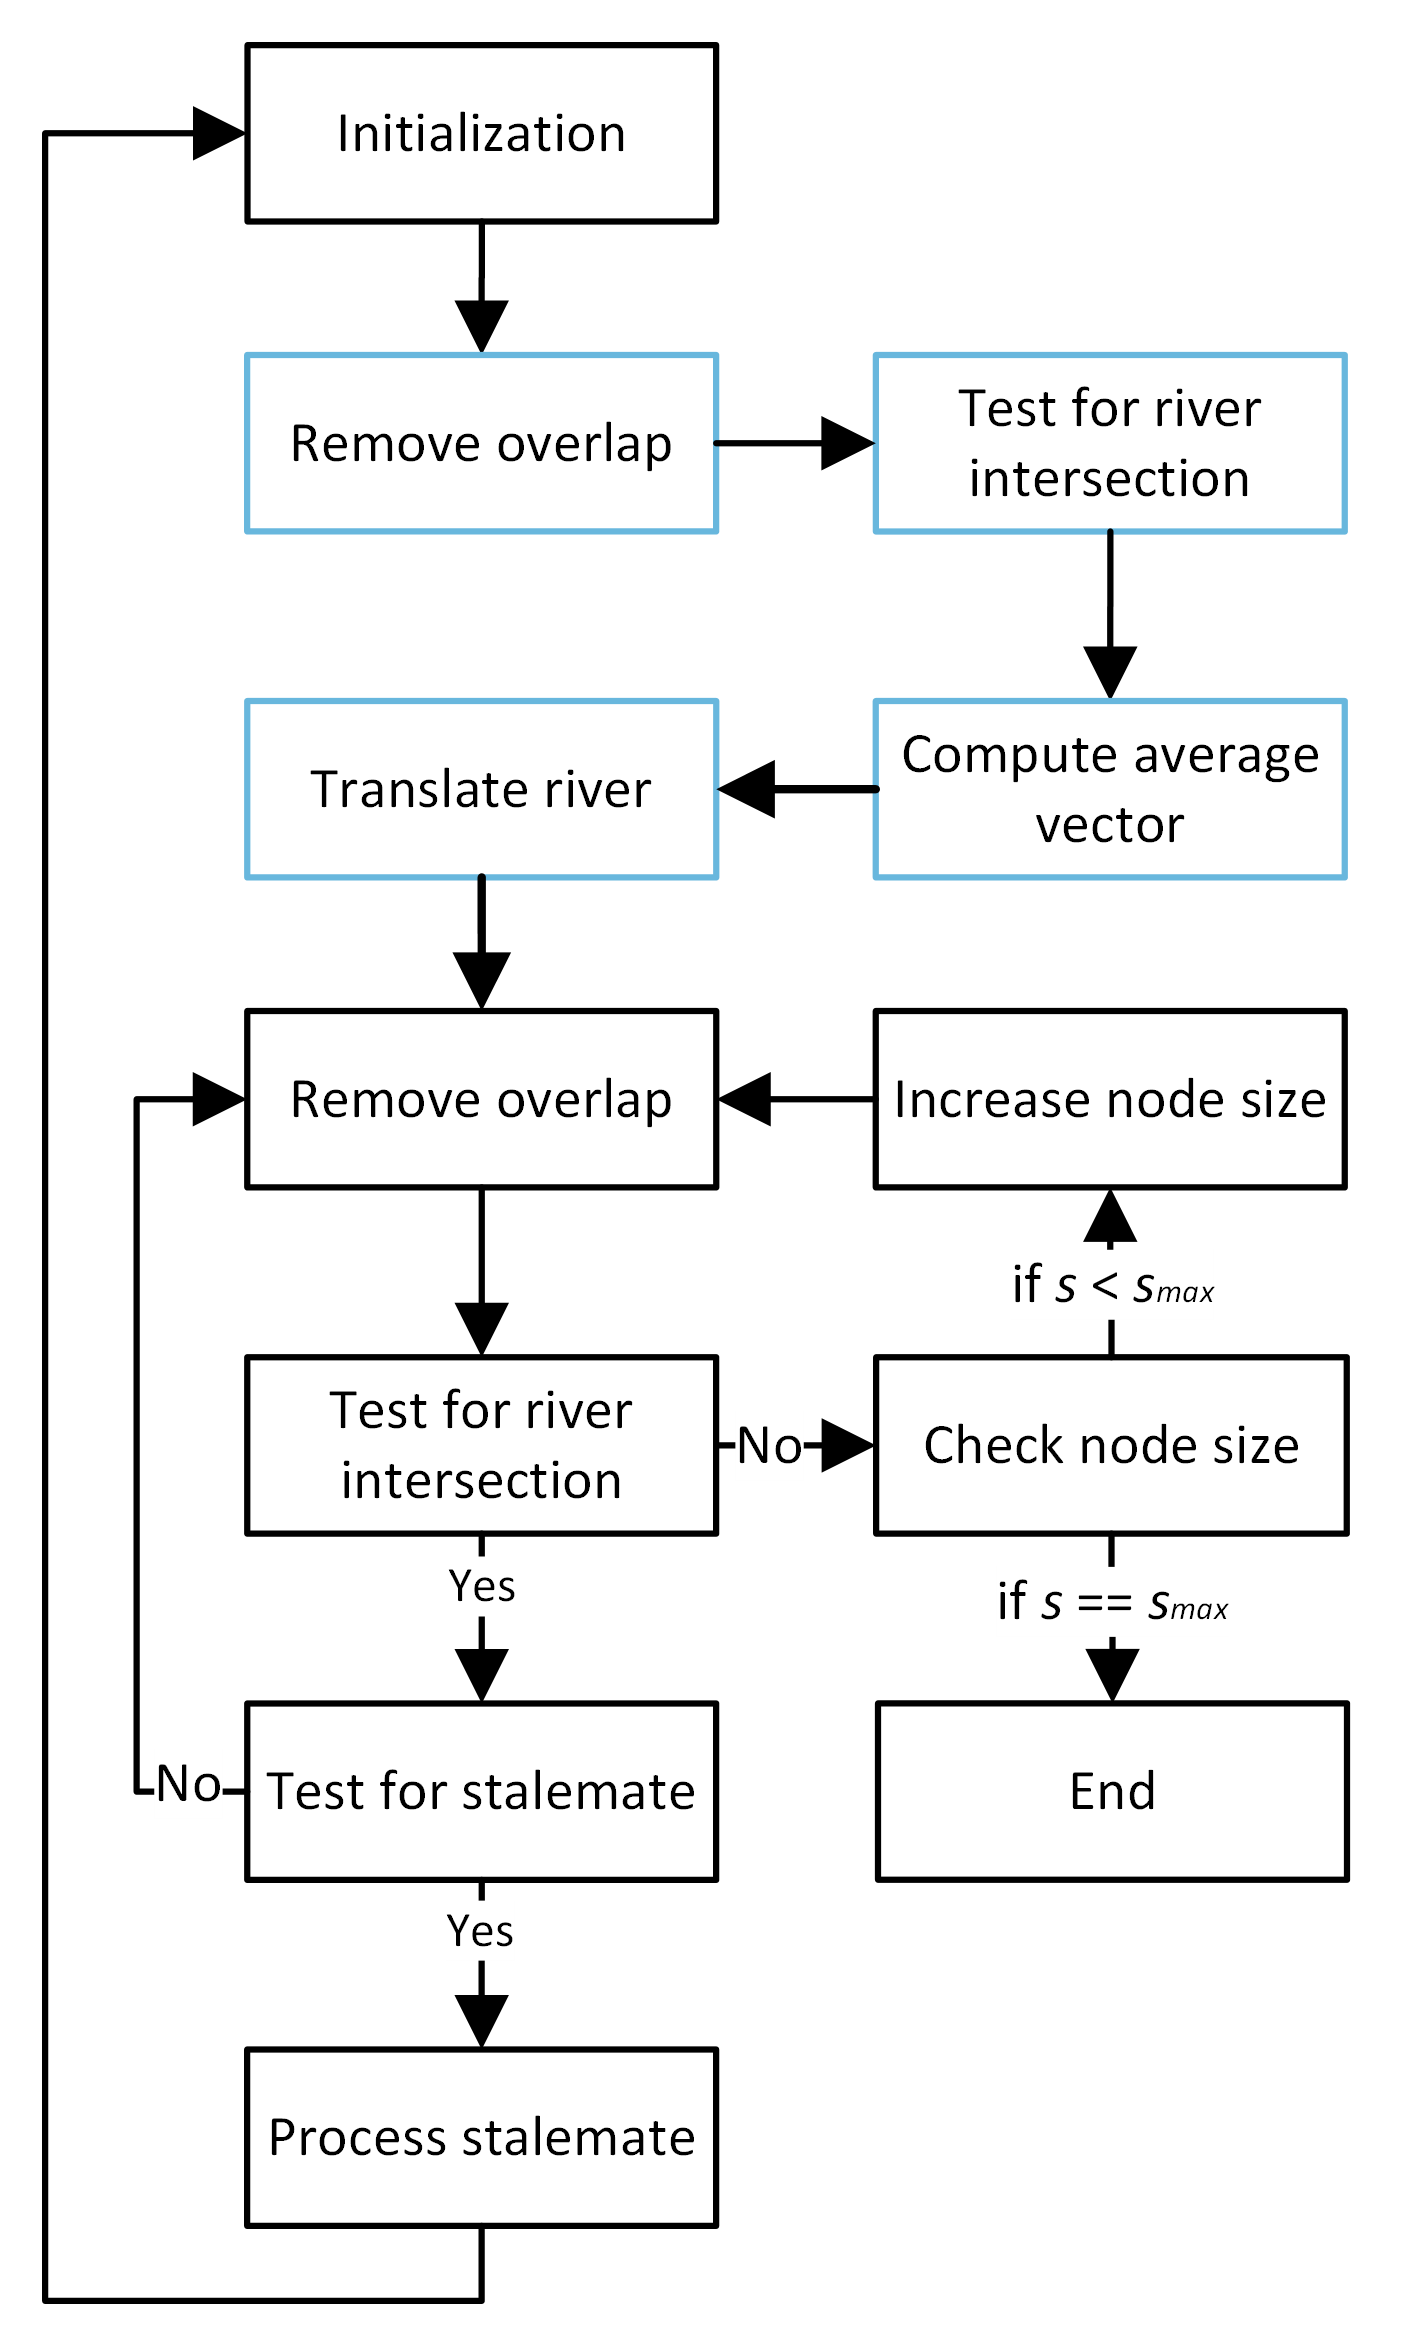
\includegraphics[width=\columnwidth]{figure/flowchart.png}
    \caption{A flowchart showing the abstraction of our layout algorithm.}
    \label{fig:flowchart}
\end{figure}
}

\algoref{alg:UpdateNodePosition} and \figref{fig:flowchart} provide an overview of our algorithm. \textbf{Initialization:} We first load and render the CCG geospatial boundaries. For each CCG we compute the centroid and represent it using a small square node with $ \nodeSize $ as the initial size. \textbf{Node layout:} The basic algorithm is as follows: we first apply the Fast Node Overlap Removal (VPSC) algorithm \cite{dwyer2006fast} repeatedly to remove overlaps. We chose VPSC over other node overlap removal algorithms since VPSC is able to provide spread minimization and node movement minimization while maintaining a good level of global shape preservation \cite{chen2020Node}. During each iteration, we compute node trajectories (See \algoref{alg:check river intersection}) and translate nodes to their new position. Nodes that cross a river are translated back to their previous position. This procedure ends when 1) no node overlap is present; 2) no nodes cross a river. We then increase $ \nodeSize $ by one pixel and repeat the algorithm until the max node size $ \nodeSizeMax $ is reached. \new{The size growing process provides a stability in the layout and minimizes geographical errors.}

% \begin{noindent}

\begin{algorithm}[tb!]
    \caption{Procedure to update node positions by removing overlap and prevent nodes from crossing rivers.}\label{alg:UpdateNodePosition}
    \textbf{Global variables:} \\
    $ \nodeList \gets $ a list of nodes representing CCGs \\
    $ \nodeSize \gets $ the current size of all nodes \\
    $ \nodeSizeMax \gets $ the maximum size of a node \\
    $ \stalemateMax \gets $ the maximum number of iterations indicating a stalemate \\

    \textbf{Local variables:} \\
    $ \nodeListVPSC \gets $ a list of nodes representing CCGs after VPSC \\
    $ \crossRiver \gets $ boolean indicating a node crossed a river \\
    $ \nodeListEach \gets $ a node in $ \nodeList $ \\
    $ \nodeListEachPrevious \gets $ the previous position of $ \nodeListEach $\\
    $ \nodeListVPSCEach \gets $ a node in $ \nodeListVPSC $, which is the next position of $ \nodeListEach $ after VPSC \\

    \begin{algorithmic}[1]
        \Procedure{UpdateNodePosition}{}
        \While{$ \nodeSize < \nodeSizeMax $}

            \State $ \nodeListVPSC \gets $ RunVPSC ($ \nodeList $)

            \ForEach {$ \nodeListVPSCEach \in \nodeListVPSC $}

                \If {\Call{TranslateNode}{$ \nodeListEach, \nodeListVPSCEach $}}
                    \State $ \crossRiver \gets $ \Call{TestRiverIntersection}{$ \nodeListEach, \nodeListVPSCEach $}

                    \If{$ \crossRiver = True $}
                        \State $ \nodeListEachStalemate \gets \nodeListEachStalemate + 1 $

                        \If{$ \nodeListEachStalemate < \stalemateMax $}
                            \State $ \nodeListEach(x,y) \gets \nodeListEachPrevious(x,y) $
                        \Else
                            \State \Call{ProcessStalemate}{$ \nodeListEach, \nodeListVPSCEach $}
                            \State $ \nodeListEachStalemate \gets 0 $
                        \EndIf

                    \EndIf

                \EndIf

            \EndFor

            \State $ \nodeSize \gets \nodeSize ++$

        \EndWhile

        \EndProcedure
    \end{algorithmic}
\end{algorithm}


\begin{algorithm}[tb!]
    \caption{Procedure to update a single node, $ \node $'s position.}\label{alg:move position}

    \textbf{Input:} \\
    $ \node \gets $ the node \\
    $ \nodeVPSC \gets $ the node after running VPSC \\

    \textbf{Output:} \\
    Returns $ True $ if the node's position is updated. \\

    \begin{algorithmic}[1]
        \Procedure{TranslateNode}{$ \node, \nodeVPSC $}
        \If{$ \node(x,y) = \nodeVPSC(x,y) $}
            \item[] \Comment{Node position remains unchanged}
            \State \Return{$ False $}
        \EndIf

        \State $ \node(x,y) \gets \nodeVPSC(x,y) $

        \State \Return{$ True $}
        \EndProcedure
    \end{algorithmic}
\end{algorithm}

%\end{noindent}

\subsection{River Intersection Testing}

We use rivers as topological boundaries and prevent nodes from crossing them. \new{The resolution of rivers can be dynamically adjusted, as shown in \figref{fig:river resolution}}. When a node's position changes, we test if the node's trajectory intersects any segment of a river. See \algoref{alg:check river intersection}. A bounding box intersection test can be performed to reduce the number of edge intersection detections required.


{
\begin{figure}[tb!]
    \centering
    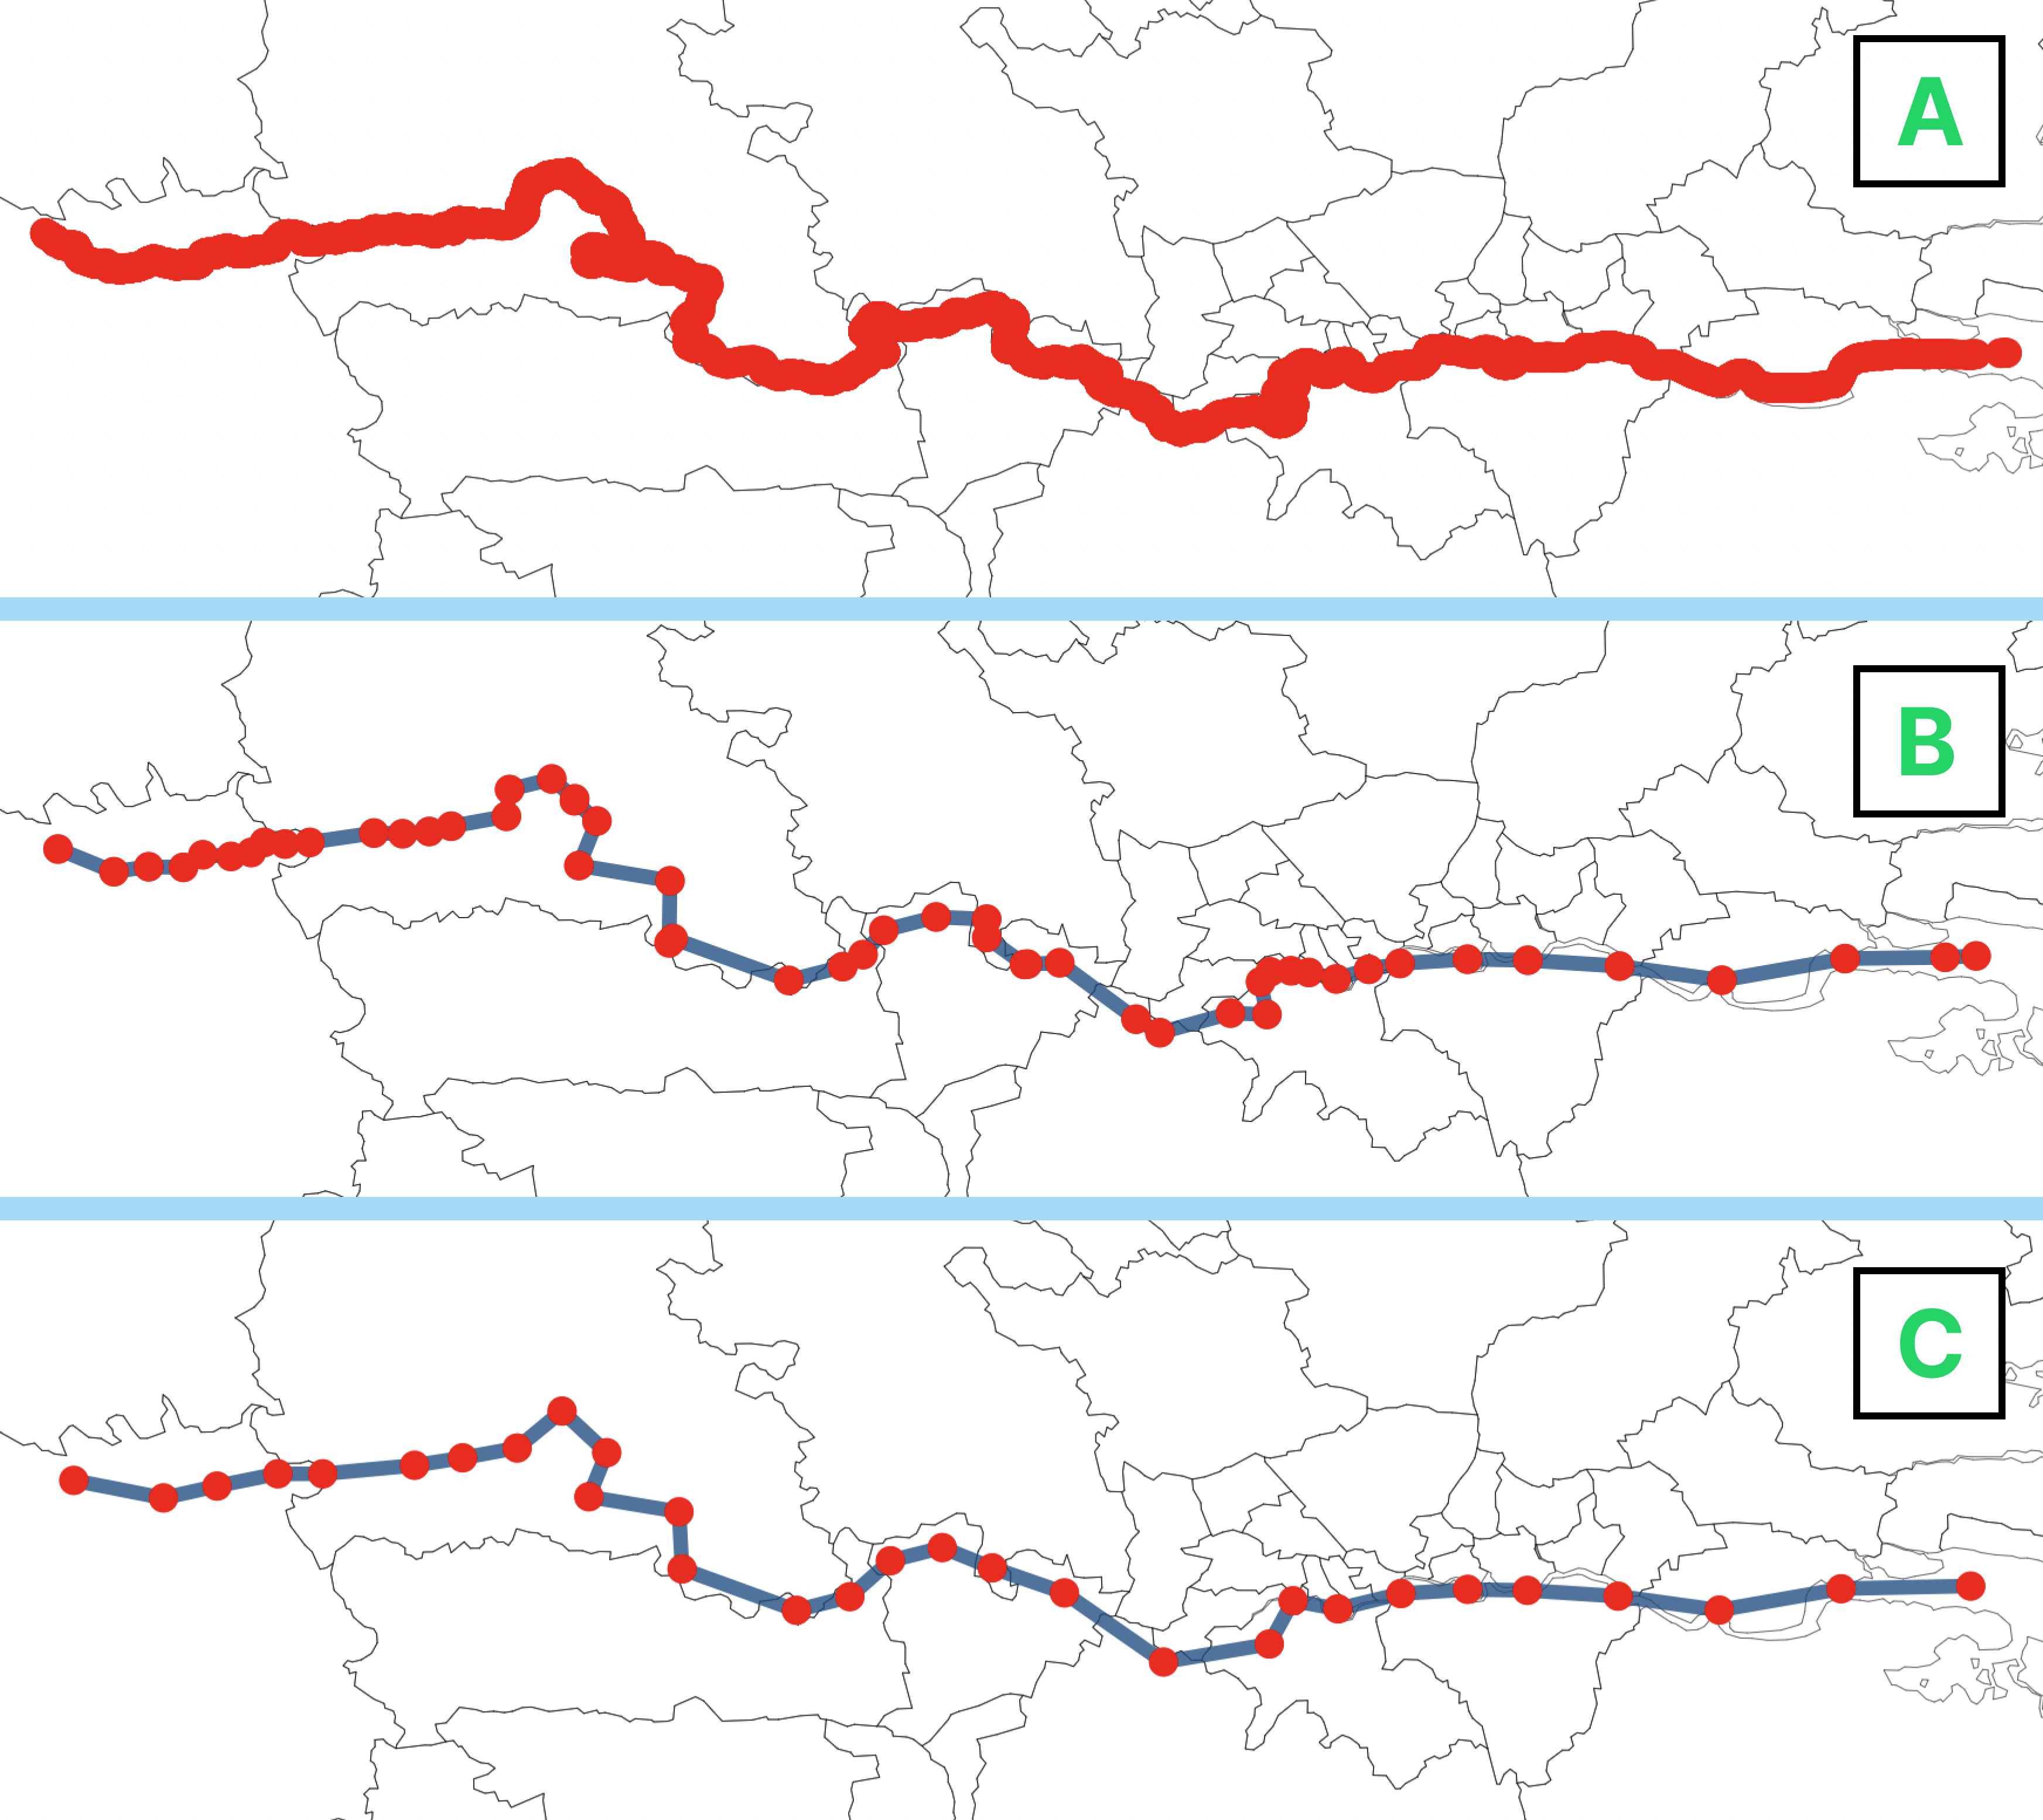
\includegraphics[width=\columnwidth]{figure/river_resolution.png}
    \caption{The resolution of rivers can be dynamically adjusted. The top figure shows River Thames at its original resolution. The bottom figure shows the river with a 60\% reduction in resolution. The reduced resolution preserves the majority of River Thames' original shape and improves the performance of our river intersection tests.}
    \label{fig:river resolution}
\end{figure}
}

% \begin{noindent}
\begin{algorithm}[tb!]
    \caption{Procedure to test if a node, $ \node $ crosses a river.}\label{alg:check river intersection}
    \textbf{Input:} \\
    $ \node \gets $ the node \\
    $ \nodeVPSC \gets $ the node after running VPSC \\

    \textbf{Output:} \\
    Returns $ True $ if the node crosses a river. \\

    \textbf{Global variables:} \\
    $ \riverEdgeList \gets $ a list of river edges \\

    \textbf{Local variables:} \\
    $ \nodeBoundingBox, \riverEdgeBoundingBoxEach \gets $ the bounding boxes for $ \nodeLineNV $ and $ \riverEdgeListEachLine $ \\
    $ \riverEdgeListEachLine \gets $ a river edge in $ \riverEdgeList $ \\ 
    % $ \boundingBoxInt \gets $ boolean indicating $ \nodeBoundingBox $ intersects $ \riverEdgeBoundingBoxEach $ \\
    % $ \nodeEdge \gets $ the edge for $ \node $\\
    % $ \edgeBoxInt \gets $ boolean indicating $ \nodeEdge $ intersects $ \riverEdgeListEach $ \\

    \begin{algorithmic}[1]
        \Procedure{TestRiverIntersection}{$ \node, \nodeVPSC $}
        
        \ForEach{$ \riverEdgeListEachLine \in \riverEdgeList $}
            \State $ \nodeBoundingBox \gets $ GetBoundingBox ($ \nodeLineNV $)
            \State $ \riverEdgeBoundingBoxEach \gets $ GetBoundingBox ($ \riverEdgeListEachLine $)
            % \State $ \boundingBoxInt \gets $ TestIntersection ($ \nodeBoundingBox, \riverEdgeBoundingBoxEach $)
            % \If{$ \boundingBoxInt = True $}

            \If{$ \nodeBoundingBox ~intersect~ \riverEdgeBoundingBoxEach = True $}
                \If{$ \nodeLineNV ~intersect~ \riverEdgeListEachLine = True $}
                    \State \Return{$ True $}
                \EndIf
            
                \EndIf
        \EndFor
        
        \State \Return{$ False $}
        \EndProcedure
    \end{algorithmic}
\end{algorithm}
%\end{noindent}

\subsection{Detecting Stalemates}

As the VPSC always tries to produce an optimal node layout where node distribution and translation are minimized, a node might be repeatedly translated between two positions due to river intersection and congestion, creating a stalemate situation, as shown in \figref{fig:stalemate}. In order to create space for VPSC to generate a new layout, we introduce a parameter, $ \stalemateMax $, to test for stalemate. If a node is translated between two positions for more than $ \stalemateMax $ iterations, it is considered to be in a stalemate. A stalemate triggers a corridor derivation, {a corridor is a rectangle with a width of $ \CorridorWidth $ and a length of $ \CorridorLength $, in the direction of the node $ \node $'s previous and current position, denoted $ \nodeVectorPC $ }, all enclosed nodes are then translated in the same direction and by the distance of that vector to alleviate the congestion.

{
\begin{figure}[tb!]
    \centering
    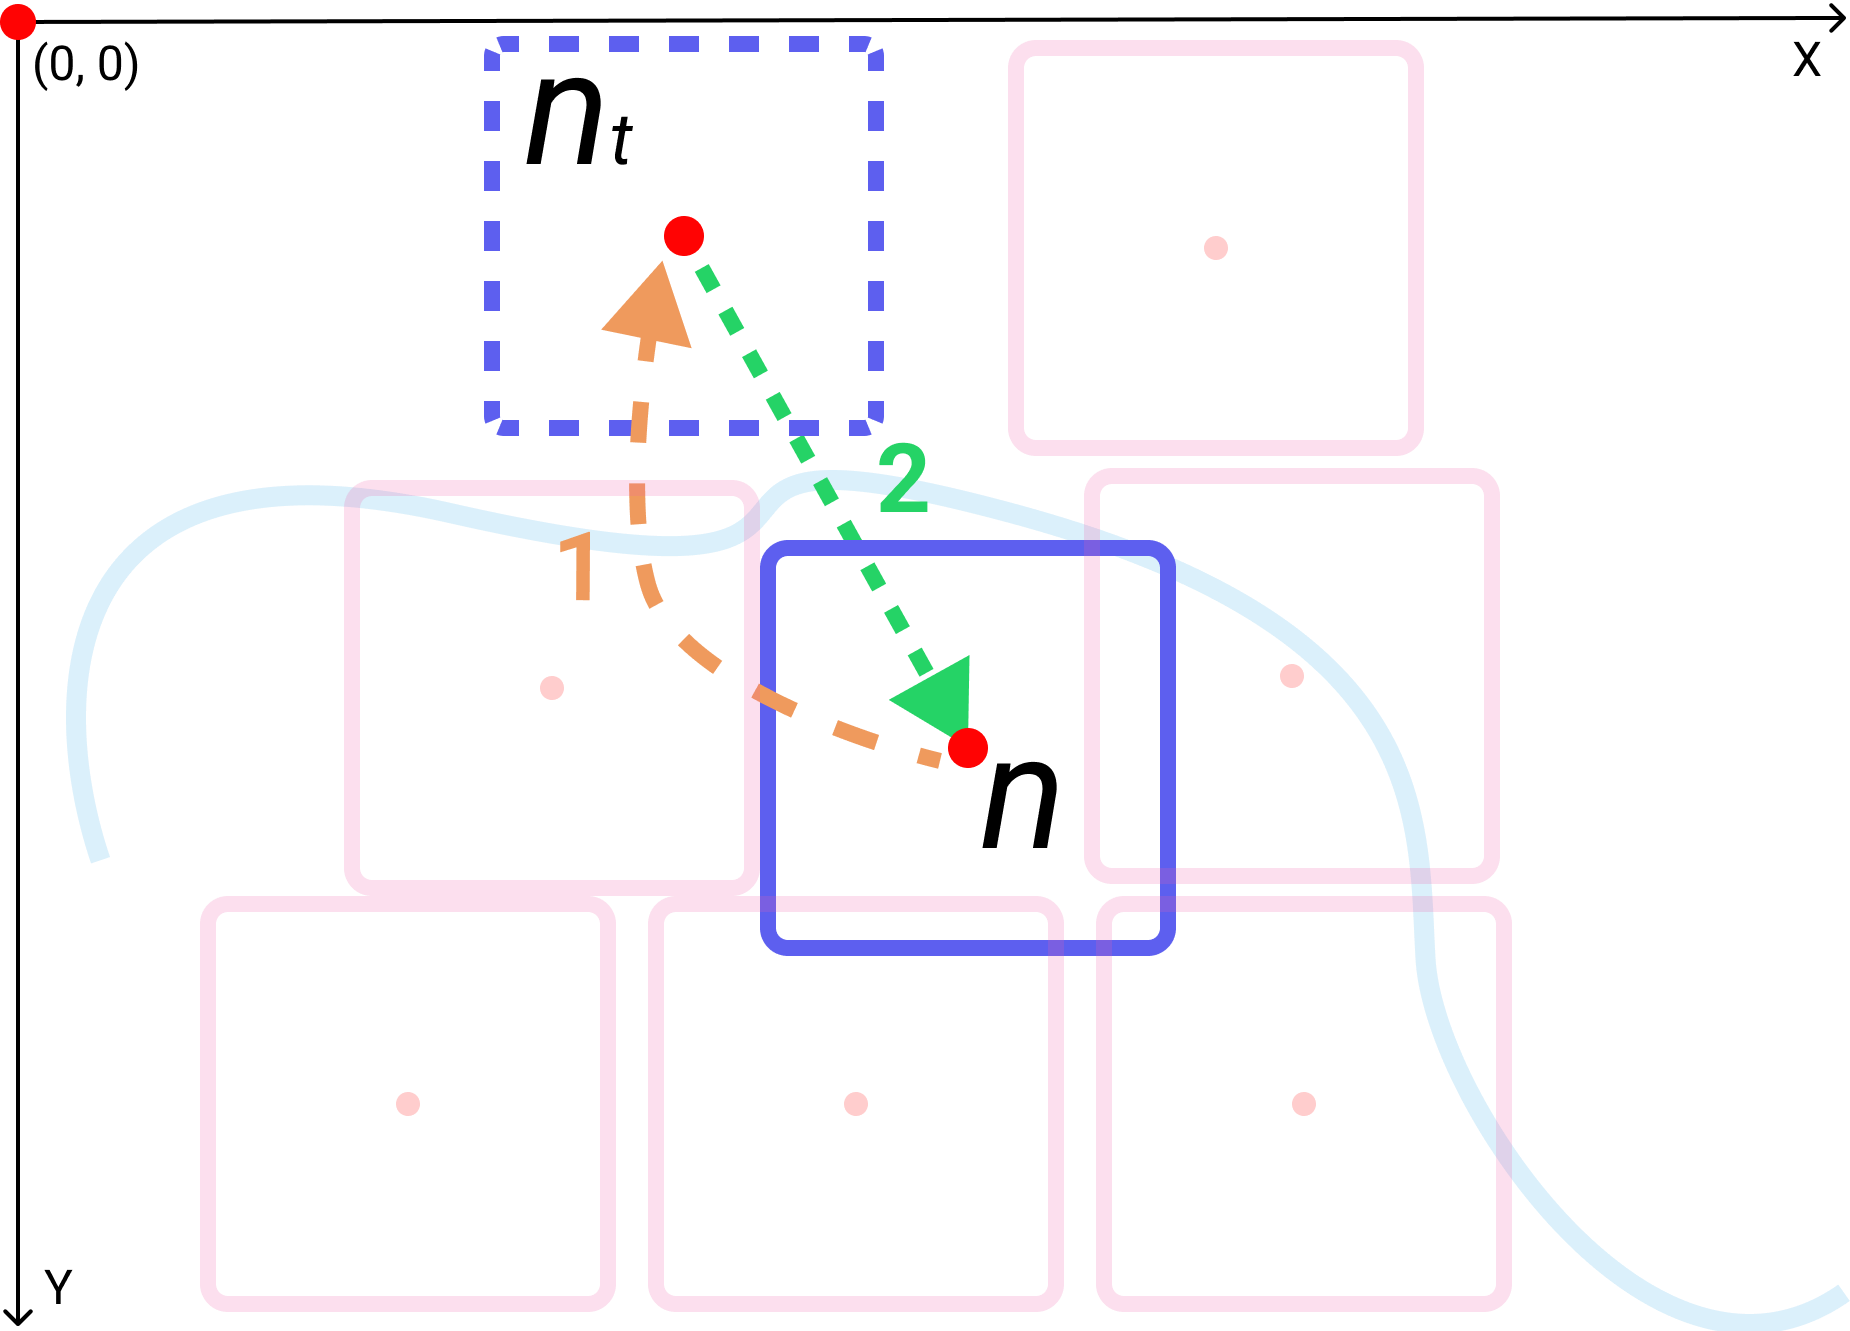
\includegraphics[width=\columnwidth]{figure/stalemate.png}
    \caption{A stalemate situation is when a node repeatedly translates between two positions (A and B) for more than $ stalemate $ iterations. }
    \label{fig:stalemate}
\end{figure}
}

{
\begin{figure}[tb!]
    \centering
    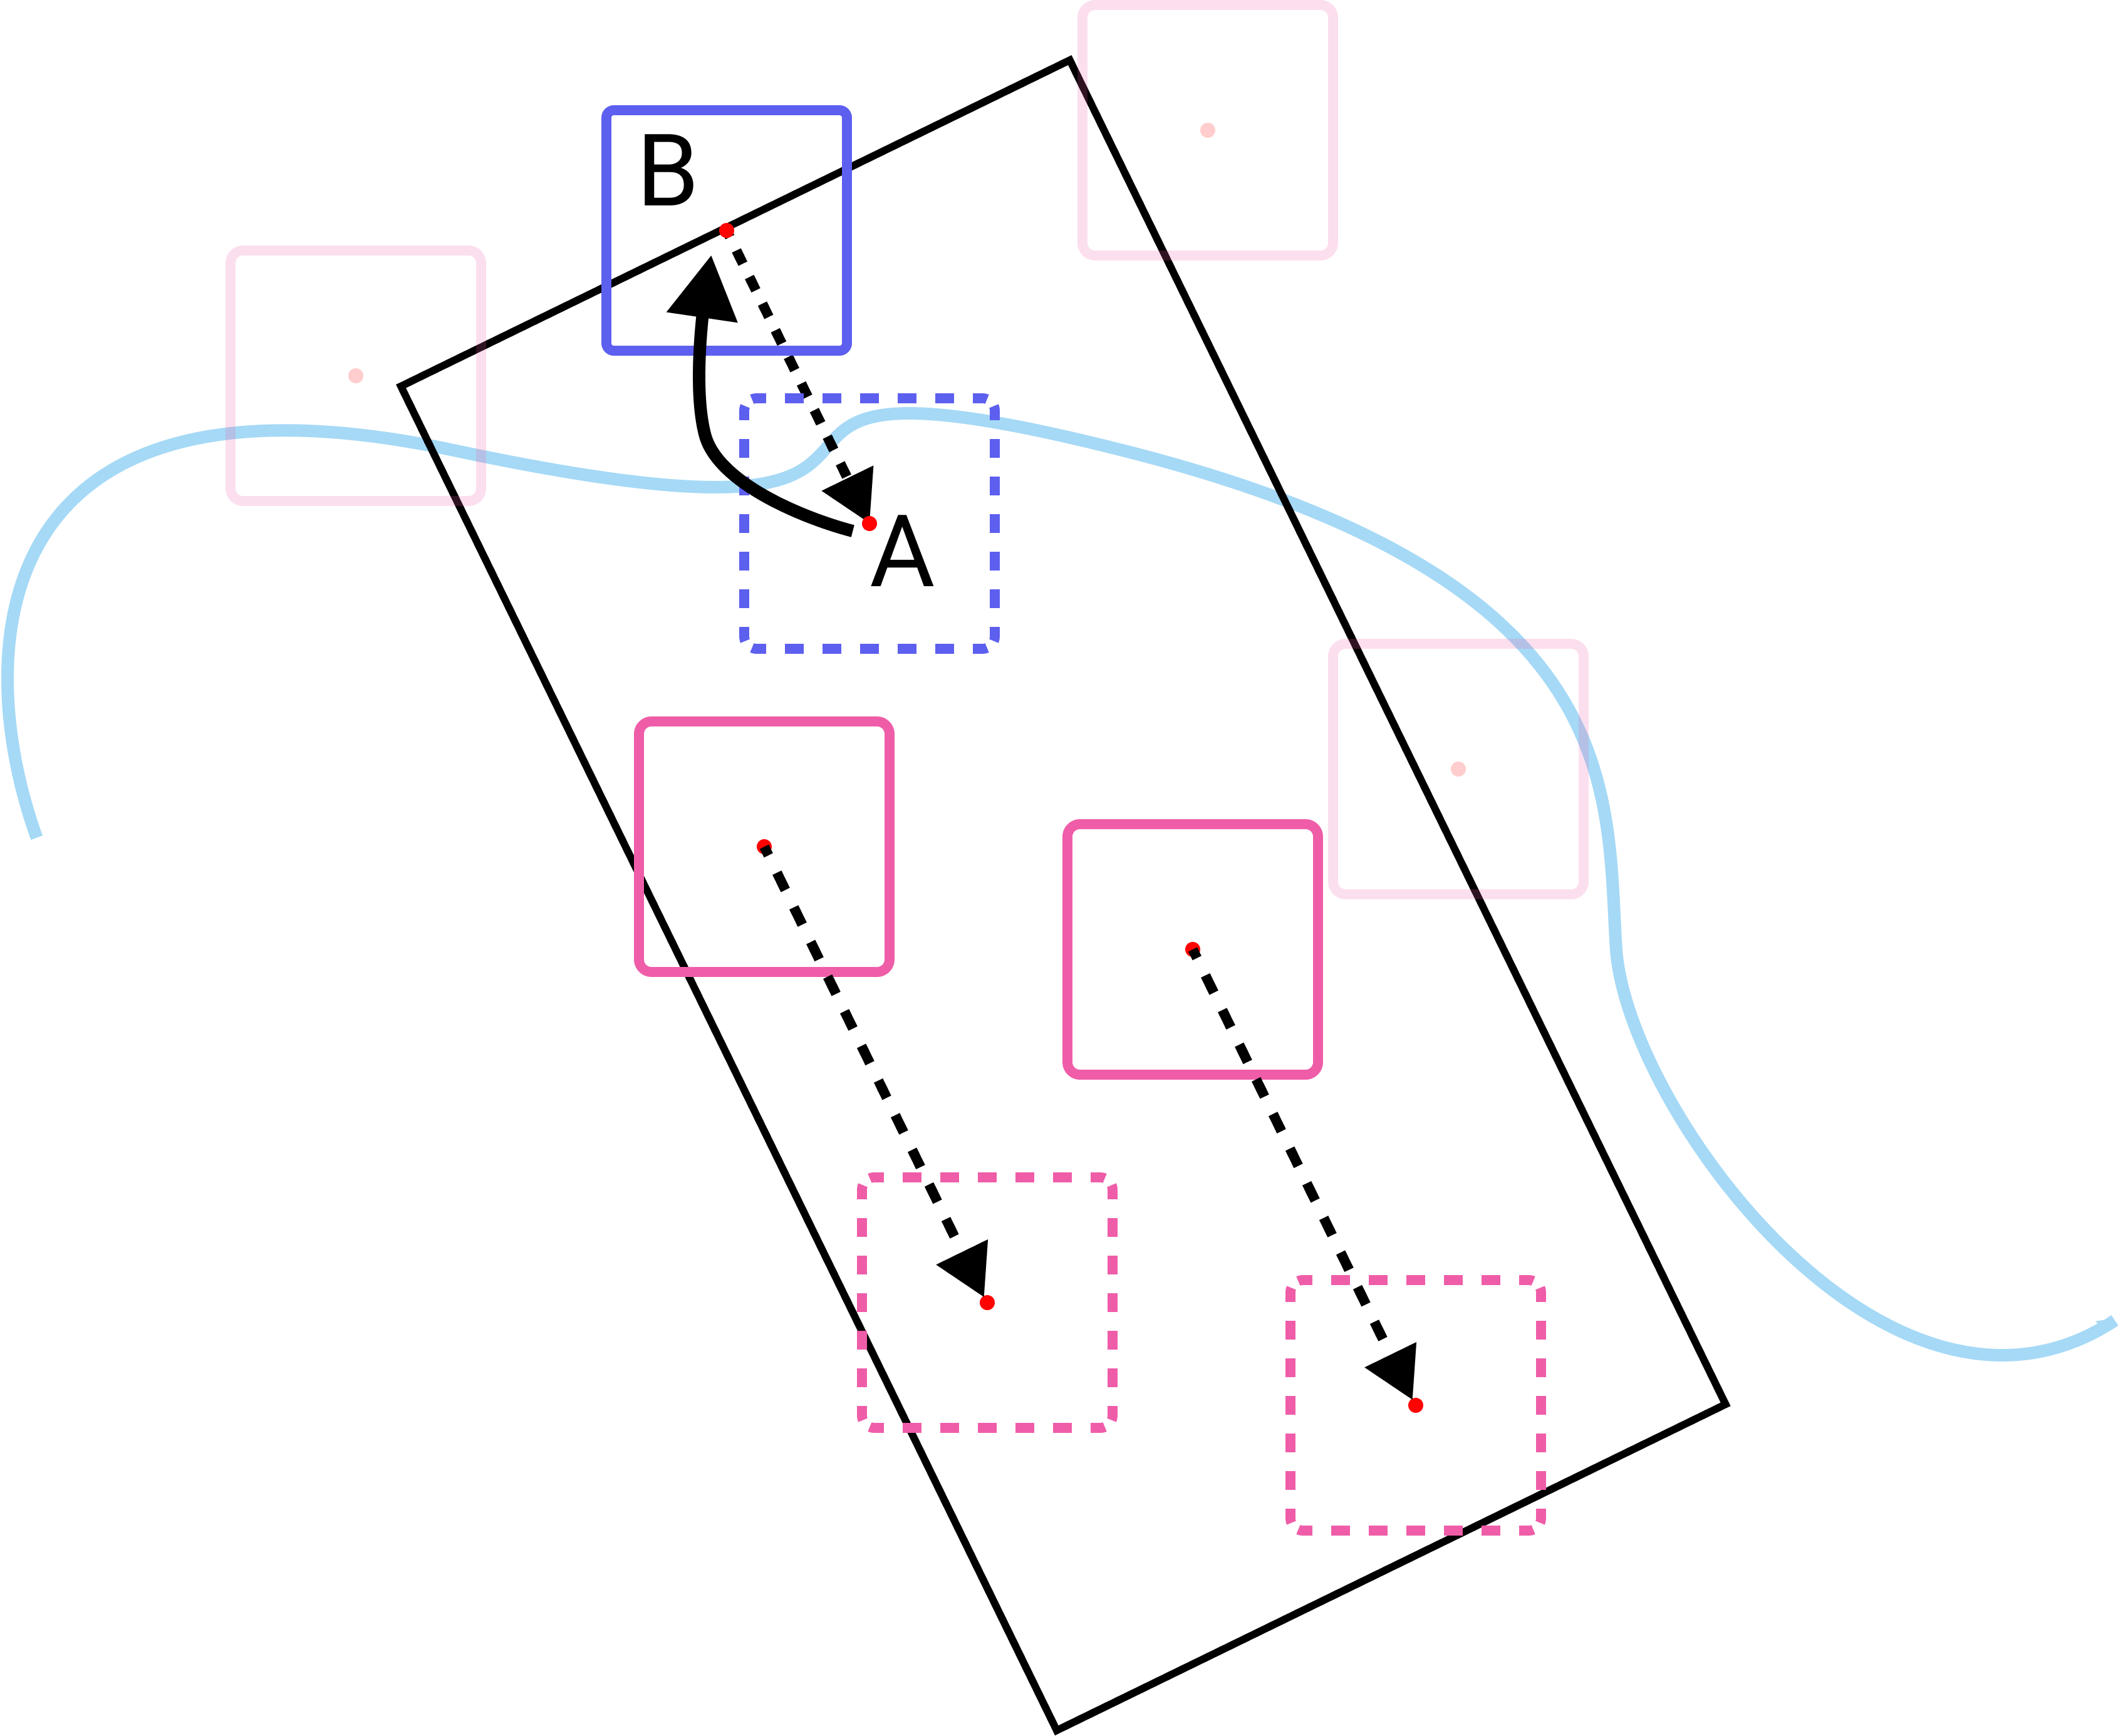
\includegraphics[width=\columnwidth]{figure/corridor.png}
    \caption{When a stalemate occurs, a corridor (black rectangular) is derived based on the current (A) and previous (B) positions of the node that crossed a river, as described in \algoref{alg:derive corridor}. All nodes within the corridor are moved by $ d $ units in the direction of $ \Vector{B}{A} $, e.g, A is moved to C. }
    \label{fig:corridor}
\end{figure}
}

% \begin{noindent}

\begin{algorithm}[tb!]
    \caption{Procedure to derive a corridor to translate enclosed nodes. We use an SVG canvas, where the point of origin (0,0) is located at the top left corner, with the x-axis extending to the right and the y-axis extending downwards.}\label{alg:derive corridor}

    \textbf{Input:} \\
    $ \node \gets $ the node used to derive the corridor \\

    \textbf{Global variables:} \\
    $ \nodeSize \gets $ the current size of all nodes \\
    $ \CorridorLength \gets $ the length of a corridor \\
    $ \CorridorWidth \gets $ the width of a corridor \\

    \textbf{Local variables:} \\
    $ \nodePrevious \gets $ the previous position of $ \node $ \\
    $ \PointP \gets $ the point extending $ \nodeVectorPC $ such that $ \nodeLineWidthNpP = \CorridorLength $\\
    $ \EdgeParallelA, \EdgeParallelB \gets $ the edges parallel to $ \nodeLineNpP $ \\
    $ corridor \gets $ a rectangle formed by $ \EdgeParallelA $ and $ \EdgeParallelB $ \\

    \begin{algorithmic}[1]
        \Procedure{ProcessStalemate}{$ \node $}
            \State TranslateNode ($ \node $)

            \State $ \PointP \gets $ \Call{DerivePoint}{$ \nodeVectorPC $, $ \CorridorLength $}

            \State $ \EdgeParallelA \gets $ \Call{DeriveParallelEdge}{$ \nodeVectorNpP $, $ \frac{\CorridorWidth}{2} $}

            \State $ \EdgeParallelB \gets $ \Call{DeriveParallelEdge}{$ \nodeVectorNpP $, $ -\frac{\CorridorWidth}{2} $}

            \State $ corridor \gets
                \begin{bmatrix}
                    \EdgeParallelA.start &
                    \EdgeParallelA.end \\

                    \EdgeParallelB.start &
                    \EdgeParallelB.end \\
                \end{bmatrix} $

                % TODO: calculate the vector once and use it for all nodes
            \ForEach{$ \nodeInCorridorEach $ inside $ corridor $}
                \State $ \nodeInCorridorEachDx \gets \nodeInCorridorEach.x - \nodeInCorridorEach.previous.x $

                \State $ \nodeInCorridorEachDy \gets \nodeInCorridorEach.y - \nodeInCorridorEach.previous.y $

                \State $ hyp \gets \sqrt{(\nodeInCorridorEachDx)^2 +(\nodeInCorridorEachDy)^2} $

                \State $ \nodeInCorridorEach.next \gets $ \Call{DerivePoint}{$ \Vector{\nodeInCorridorEach.previous}{~\nodeInCorridorEach} $, $ hyp + s $}

                \State TranslateNode ($ \nodeInCorridorEach $, $ \nodeInCorridorEach.next $)

            \EndFor
        \EndProcedure
    \end{algorithmic}
\end{algorithm}

%\end{noindent}

% \begin{noindent}

    \begin{algorithm}[tb!]
        \caption{Procedure to derive a point based an edge and a distance.}\label{alg:derive corridor point}
        \textbf{Input:} \\
        $ \Edge \gets $ the edge used to derive the new point \\
        $ \Distance \gets $ the distance between $ \PointP $ and $ \EdgeStart $ \\

        \textbf{Output:} \\
        A point, $ \PointP $, that is distance $ \Distance $ away from $ \EdgeStart $. \\
    
        \textbf{Local variables:} \\
        $ \dx, \dy \gets $ the differences in $ x, y $ for $ \EdgeStart $ and $ \EdgeEnd $ \\
    
        \begin{algorithmic}[1]
            \Procedure{DerivePoint}{$ \Edge $, $ \Distance $}
                \State $ \dx \gets \EdgeStart.x - \EdgeEnd.x $
    
                \State $ \dy \gets \EdgeStart.y - \EdgeEnd.y $
    
                \State $ \PointP.x \gets \frac{\dx}{\sqrt{\dx^2 + \dy^2}} \cdot \Distance $
    
                \State $ \PointP.y \gets \frac{\dy}{\sqrt{\dx^2 + \dy^2}} \cdot \Distance $
    
            \State \Return{$ \PointP $}
    
            \EndProcedure
    
        \end{algorithmic}
    \end{algorithm}
    
    %\end{noindent}


% \begin{noindent}

\begin{algorithm}[tb!]
    \caption{Procedure to derive an edge, $ \EdgeParallel $, that is parallel to $ \Edge $ with a distance of $ \Distance $.}\label{alg:derive corridor edge}

    \textbf{Input:} \\
    $ \Edge \gets $ the edge used to derive the parallel edge $ \EdgeParallel $ \\
    $ \Distance \gets $ the distance between $ \Edge $ and $ \EdgeParallel $ \\

    \textbf{Output:} \\
    An edge, $ \EdgeParallel $, that is parallel to $ \Edge $ with a distance of $ \Distance $. \\

    \textbf{Local variables:} \\
    $ \dx, \dy \gets $ the differences in $ x, y $ for $ \EdgeStart $ and $ \EdgeEnd $ \\
    $ \Scale \gets $ the scale of $ \frac{\Distance}{\sqrt{\dx^2 + \dy^2}} $ \\

    \begin{algorithmic}[1]
        \Procedure{DeriveParallelEdge}{$ \Edge $, $ \Distance $}
            \State $ \dx \gets \EdgeStart.x - \EdgeEnd.x $

            \State $ \dy \gets \EdgeStart.y - \EdgeEnd.y $

            \State $ \Scale \gets \frac{\Distance}{\sqrt{\dx^2 + \dy^2}} $

            \State $ \EdgeParallel.start.x \gets \Scale \cdot -\dy + \EdgeStart.x $

            \State $ \EdgeParallel.start.y \gets \Scale \cdot \dx + \EdgeStart.y $

            \State $ \EdgeParallel.end.x \gets \Scale \cdot -\dy + \EdgeEnd.x $

            \State $ \EdgeParallel.end.y \gets \Scale \cdot \dx + \EdgeEnd.y $

        \State \Return{$ \EdgeParallel $}

        \EndProcedure

    \end{algorithmic}
\end{algorithm}

%\end{noindent}